\chapter{Optimizing SteelEagle Performance}

As explained in \cref{sec:overview}, the performance of the SteelEagle system
determines its versatility. A drone that is slow to react will be unable to
effectively navigate obstacle-dense environments. The chances of the drone
losing track of a fast on-ground target that is moving erratically increases
substantially if the drone is slow in keeping the target centered in its view.
Given the importance of performance, this chapter details how performance is
defined for SteelEagle, how it is measured, and work done to identify
performance bottlenecks and optimize the system.

\cref{sec:exp1} describes initial efforts to optimize the system that yielded a
more than two-fold reduction in drone-to-cloudlet latency, discovering negative
scale-out attributes of FFmpeg, a video decoding library.  \cref{sec:exp2}
describes subsequent efforts to establish a more systematic approach to
profiling SteelEagle, which found the encoding of the RTSP video stream
generated by the drone to be the biggest contributor to latency.

\begin{figure}[htbp]
\centerline{\includegraphics[width = .5\textwidth]{figs/fig-simplified-arch.png}}
\caption{SteelEagle Edge Offload Pipeline}
\label{fig:simplified-arch}
\end{figure}

\section{How is performance defined in SteelEagle?}
\label{sec:steeleagle-performance-def}

The performance of SteelEagle is determined by the end-to-end latency and
throughput of the system. \cref{sec:overview} explained how drones in
SteelEagle are treated as thin clients, with the use of a communications relay
to make up for the lack of cellular connectivity on commerical-off-the-shelf
(COTS) drones. The sensor stream from the drone is forwarded to the
communications relay over Wi-Fi, which in turn forwards it to the cloudlet over
4G LTE. After performing inference on the received data, the cloudlet sends
back piloting commands to the drone, via a hop through the communications relay
(\cref{fig:simplified-arch}). As a result, the end-to-end performance is
determined by several components of the pipeline:
\begin{enumerate}
    \item[(a)] On-drone sensing
    \item[(b)] On-drone pre-processing
    \item[(c)] Tranmission to cloudlet
    \item[(d)] Cloudlet processing
    \item[(e)] Transmission to drone
    \item[(f)] Drone post-processing
    \item[(g)] Drone actuation
\end{enumerate}

Each of these components has a latency associated with it, and a throughput
that it is capable of. The performance of components (a), (b), (f), and (g) is
fixed for a given drone. Factors such as the drone camera's sensor readout time
and shutter speed used affect the frame capture latency, and thus determine the
performance of component (a). Component (b) consists of any processing of the
sensor data before it is transmitted from the drone. The generation of an H.264
stream, for instance, adds latency since the compression process is
computationally intensive, involving analysis of deltas between successive
frames.

For components (c) and (e), performance is determined by the cellular network
used for communication between the relay and the cloudlet. While there is
variance associated with the performance of these components, factors such as
the number of network hops, distance between the relay to the cloudlet, and the
network signal strength available to the relay largely determine the 99th
percentile value of their latency and throughput over a longer period of time.
The performance of component (d) can vary largely based on whether decoding of
the drone stream data is required and type of inferencing that is performed. A
DNN with a complex architecture, for instance, can take much longer for
inference than a traditional computer vision approach. The same inference can
also take less time on a more powerful cloudlet.

\begin{figure}[htbp]
\definecolor{observe-color}{RGB}{175,208,149}
\definecolor{orient-color}{RGB}{255, 255, 166}
\definecolor{decide-color}{RGB}{255,170,149}
\definecolor{act-color}{RGB}{224,194,205}
\centering
\includegraphics[width = .6\textwidth]{figs/fig-ooda-loop.pdf}\\
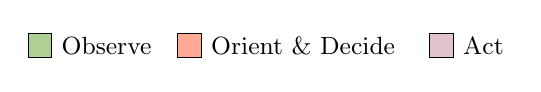
\begin{tikzpicture}
    \draw[fill=observe-color] (1.0,0) rectangle (1.3,0.3);
    \node[right] at (1.3,0.15) {\small Observe};

    \draw[fill=decide-color] (2.9,0) rectangle (3.2,0.3);
    \node[right] at (3.2,0.15) {\small Orient \& Decide};

    \draw[fill=act-color] (6.1,0) rectangle (6.4,0.3);
    \node[right] at (6.4,0.15) {\small Act};
\end{tikzpicture}
\caption{Mapping the SteelEagle pipeline to the OODA loop}
\label{fig:ooda-mapping}
\end{figure}

\Cref{fig:ooda-mapping} shows how these components can be mapped to the various
stage of the OODA pipeline. The ``Observe'' phase includes components (a), (b),
and (c). Components (d) maps to the ``Orient'' and ``Decide'' phases. Finally,
components (e), (f), and (g) correspond to the ``Act'' phase.

\section{Measuring the performance of the SteelEagle pipeline}
\label{sec:steeleagle-performance-measurement}

Benchmarking the performance of SteelEagle is challenging since it uses COTS
drones that restrict modification of its onboard software. The inability to add
software instrumentation on the drone makes it difficult to determine when a
given frame was transmitted from the drone. To circumvent this restriction,
Bala et al adapted the technique George et al used for measuring
motion-to-photon latency in augmented reality \cite{george20}.


\begin{figure}[htbp]
\centerline{\includegraphics[width = .8\textwidth]{figs/mtp_pipeline.png}}
\caption{Technique for measuring end-to-end latency}
\label{fig:latency-measuring-technique}
\end{figure}
As shown in \cref{fig:latency-measuring-technique}, the drone is kept
stationary in a lab setting with its camera pointed at a display connected to
the cloudlet showing the current Unix timestamp at millisecond granularity. The
drone captures images containing the timestamp displayed and transmits them to
the cloudlet through the SteelEagle pipeline. The cloudlet records the
timestamp at which it receives each frame, storing the frame along with this
timestamp. These saved frames are then
post-processed to compute the difference between the timestamps shown in each
frame and the timestamps at which they were received at the cloudlet. This
difference corresponds to the latency of components (a) through (d).

\section{Experiment 1: Optimizing SteelEagle Video Decoding}
\label{sec:exp1}

\begin{figure}[htbp]
\centerline{\includegraphics[width = .4\textwidth]{figs/bala_latency.pdf}}
\caption{Original SteelEagle Latency \cite{bala2024}}
\label{fig:steeleagle-original-latency}
\end{figure}

\begin{figure}[b]
    \centering
    \begin{subfigure}[t]{0.45\textwidth}
        \centering
        \includegraphics[height=1in]{figs/parrot-anafi.pdf}
        \caption{Parrot Anafi}
        \label{fig:parrot-anafi}
    \end{subfigure}
    \begin{subfigure}[t]{0.45\textwidth}
        \centering
        \includegraphics[height=1in]{figs/onion-omega.png}
        \caption{Onion Omega}
        \label{fig:onion-omega}
    \end{subfigure}
    \caption{The commerical-off-the-shelf components used in the SteelEagle system}
\end{figure}

The starting point of our investigation into the performance of the SteelEagle
system is the mean drone-to-cloudlet latency of 933 ms reported by Bala et al
in their benchmarking of the SteelEagle system
(\cref{fig:steeleagle-original-latency}). This includes the ``Observe'' and
``Orient \& Decide'' components of the OODA pipeline, components (a) through
(d) in \cref{fig:ooda-mapping}.  The latency was obtained using the Parrot
Anafi drone (\cref{fig:parrot-anafi}), which transmits a 720p H.264 RTSP stream
at 30 FPS over UDP from its monocular camera.  The Anafi uses a slice encoding
and intra-refresh scheme that disperses keyframe slices across multiple network
packets \cite{anafi_white_paper}. To reduce network bandwidth requirements, it
generates an H.264 compressed video stream using onboard hardware from the raw
frames that it obtains from its camera. Consequently, decoding of this H.264
stream is required to obtain individual video frames.  The setup uses the Onion
Omega 2 LTE (\cref{fig:onion-omega}) as a network gateway to allow the Anafi to
reach the cloudlet over LTE, since the Parrot Anafi lacks cellular
connectivity.

The technique to measure latency described in
\cref{sec:steeleagle-performance-measurement} does not provide a granular
latency breakup. As a result, it is not clear from the measurements where the
bottleneck resides. As an initial approach, we measure the impact on latency
when the cloudlet location and the video decoding library used are modified. If
the latency is significantly reduced by changing a factor, we can conclude that
the bottleneck resides in the corresponding component.

\subsection{Pipeline Experimentation Parameters}

Our first experiments measure the impact on latency when the location of the
backend and the video decoding library used is changed. \Cref{tab:experiment-parameters}
summarizes the different parameters tested along these dimensions.
\begin{table}[htbp]
    \centering
    \caption{Latency Pipeline Experimentation Parameters}
    \label{tab:experiment-parameters}
    \begin{tabular}{@{}ll@{}}
        \toprule
        \textbf{Dimension} & \textbf{Parameters} \\ \midrule
        Backend Location & Cloudlet, AWS Small, AWS Big \\
        Video Decoding Library & FFmpeg, PDrAW \\ \bottomrule
    \end{tabular}
\end{table}

We now describe the details of these parameters:

\begin{itemize}

    \item \textbf{Location of backend.} Three backend locations with different
specifications, each offering varying levels of performance, are considered to
evaluate how hardware scale-up affects system latency. The SteelEagle backend
is either set up on a bare-metal server on CMU's campus, labeled ``Cloudlet'',
or on an EC2 VM in AWS East (Virginia). Two types of EC2 instances are used,
``AWS Small'' and ``AWS Big''. The CMU Cloudlet has two
Intel\textsuperscript{\textregistered} Xeon\textsuperscript{\textregistered}
E5-2699 v3 CPUs clocked at 2.30 GHz for a total of 72 vCPUs, 128GB main memory,
and an NVIDIA\textsuperscript{\textregistered}
GeForce\textsuperscript{\textregistered} GTX 1080 Ti GPU. AWS denotes a
\texttt{g4dn.xlarge} EC2 instance which has 4 vCPUs, 16GB of memory, and an
NVIDIA T4 GPU. AWS Big is a \texttt{g4dn.16xlarge} EC2 instance which has 64
vCPUs, 256GB main memory, and also an NVIDIA T4 GPU. \Cref{tab:backend-specs}
summarizes these specifications.

\begin{table}[h]
    \centering
    \caption{Specifications of Backends Used in Experiment}
    \label{tab:backend-specs}
    \begin{tabular}{@{}llll@{}}
        \toprule
        \textbf{Backend} & \textbf{vCPUs} & \textbf{Memory} & \textbf{GPU} \\ \midrule
        AWS Small & 4 & 16 GB & NVIDIA\textsuperscript{\textregistered} T4\\
        AWS Big & 64 & 256 GB & NVIDIA\textsuperscript{\textregistered} T4\\
        Cloudlet & 72 & 128 GB & NVIDIA\textsuperscript{\textregistered} GeForce\textsuperscript{\textregistered} GTX 1080 Ti\\
        \bottomrule
    \end{tabular}
\end{table}

\item \textbf{Video decoding library.} Two video decoding libraries are considered:
FFmpeg and PDrAW (pronounced ``pedro''). FFmpeg \cite{ffmpeg} is an open-source
project that offers libraries for video encoding/decoding and
multiplexing/demultiplexing. FFmpeg is known for forming a core part of the VLC
media player. We interact with FFmpeg through OpenCV~\cite{opencv}, which
offers the ability to use FFmpeg as a backend for its video capture APIs.
PDrAW \cite{pdraw} is a part of Parrot's Ground SDK software. Similar to
FFmpeg, it includes multiplexing/demultiplexing abilities and can read from the
RTSP stream generated by the Parrot Anafi drone. Unlike FFmpeg, however, PDrAW
is intended as a video player for RTSP and MP4 videos and lacks general-purpose
encoding and decoding abilities.

\end{itemize}
\subsection{Experimental Results}

\Cref{tab:latency_summary} summarizes the results obtained. For each backend
location, the latency is measured using the two different video decoding
libraries. The mean latency of 933 ms obtained by Bala et al mentioned before
used FFmpeg with the ``Cloudlet'' backend. We measured a lower mean of 888 ms
using these parameters because our experiments do not include inference time on
the cloudlet. Inference time can vary across different machine learning models,
depending on the kind of pre-preprocessing performed and architectural details
such as the number of hidden layers used.  Not including inference time, then,
allows us to focus on the contribution of other components.

\begin{table}[t]
    \centering
    \caption{Drone-to-Cloudlet SteelEagle Latency (in ms)}
    \label{tab:latency_summary}
        \sisetup{
        detect-all,
        table-number-alignment = center,
        input-decimal-markers = {.},
        group-separator={,},
        group-minimum-digits=4
    }
    \begin{tabularx}{0.6\linewidth}{@{}
        X
        c%S[table-format=3.0]
        S[table-format=3.0]
        S[table-format=3.0]
        S[table-format=3.0]
        S[table-format=4.0]@{}
    }
    \toprule
    \textbf{Configuration} & \textbf{Average} & \textbf{Median} & \textbf{p95} & \textbf{Min} & \textbf{Max} \\
    \midrule
    \multicolumn{6}{@{}l}{\textbf{Cloudlet}} \\
    FFmpeg & 888 {\small $\pm$ 30} & 887 & 917 & 838 & 1030 \\
    PDrAW   & 380 {\small $\pm$ 15} & 379 & 402 & 344 & 420 \\
    %WiFi + FFmpeg & 841.52 & 841 & 868.3 & 16.79 & 807 & 879 \\
    %WiFi + PDrAW & 340.82 & 338.5 & 373.5 & 21.82 & 298 & 419 \\
    \midrule
    \multicolumn{6}{@{}l}{\textbf{AWS Small}} \\
    FFmpeg & 536 {\small $\pm$ 75} & 521 & 600 & 473 & 936 \\
    PDrAW   & 429 {\small $\pm$ 21} & 427 & 467 & 387 & 475 \\
    \midrule
    \multicolumn{6}{@{}l}{\textbf{AWS Big}} \\
    FFmpeg & 870 {\small $\pm$ 20} & 868 & 900 & 837 & 925 \\
    PDrAW   & 367 {\small $\pm$ 20} & 365 & 392 & 327 & 416 \\
    \bottomrule
    \end{tabularx}\\
    \vspace{0.1in}
    \footnotesize
    50 samples obtained for each configuration.
\end{table}

When using FFmpeg, moving the backend from the Cloudlet to AWS Small leads to
an extreme drop in latency, with a reduction in p95 latency from 917 ms to 600
ms (\Cref{tab:latency_summary}). This amounts to a 1.5$\times$ speedup,
with an improvement of over 300 ms. \Cref{fig:box_plots} shows an interesting
trend. The latency for AWS Small, which has the weakest computation power, is
the lowest when using FFmpeg and the highest when using PDrAW.  This
discrepancy is unexpected, as we anticipate AWS Small to perform consistently
across both setups.

This led to the hypothesis that FFmpeg's performance degrades with increased
parallelism, as it struggles to scale effectively with higher CPU counts.  To
test this hypothesis, measurements were obtained by varying the number of
threads used for FFmpeg from one to six (see \Cref{fig:threads_box_plot}).  The
OpenCV option \texttt{CAP\_\allowbreak PROP\_\allowbreak N\_\allowbreak
THREADS} was used to set the number of threads used for the FFmpeg backend.
The results show that the latency increases as we increase the number of threads,
suggesting that FFmpeg suffers from negative-scale out attributes. Adding more
threads to FFmpeg hurts latency.

\begin{figure}[htbp]
\centerline{\includegraphics[width = .4\textwidth]{figs/threads_box_plot.pdf}}
\caption{Latency vs. Number of FFmpeg Threads}
\label{fig:threads_box_plot}
\end{figure}

\begin{figure}[htbp]
    \centering
    \begin{subfigure}[t]{0.45\textwidth}
        \centering
        \includegraphics[height=2.5in]{figs/ffmpeg_box_plot.pdf}
        \caption{FFmpeg}
        \label{fig:ffmpeg_box_plot}
    \end{subfigure}
    \begin{subfigure}[t]{0.45\textwidth}
        \centering
        \includegraphics[height=2.5in]{figs/pdraw_box_plot.pdf}
        \caption{PDrAW}
        \label{fig:pdraw_box_plot}
    \end{subfigure}\vspace{1mm}\\
        \footnotesize{Each box extends from the first quartile ($Q_1$) to the third quartile ($Q_3$), with a line at the median. Whiskers extend from the box to the farthest data point lying within 1.5x the inter-quartile range ($IQR = Q_3-Q_1$) from the box. Circles represent outliers. 50 samples obtained for each configuration.}
    \caption{Latency Across Backend Locations Using Different Video Decoding Libraries}
    \label{fig:box_plots}
\end{figure}

Across all backend locations, we achieve the lowest latency by replacing FFmpeg
with PDrAW for video decoding.  For CMU Cloudlet, latency reduced
from 917 ms to 402 ms by switching to PDrAW, a speedup of almost 2.3$\times$.

\begin{figure}[htbp]
\centerline{\includegraphics[width = .4\textwidth]{figs/pdraw_latency.pdf}}
\caption{Optimized SteelEagle Latency using PDrAW for Video Decoding}
\label{fig:steeleagle_optimized_latency}
\end{figure}

\section{Experiment 2: A More Structured Benchmarking Approach}
\label{sec:exp2}

\Cref{sec:exp1} covered an initial approach to benchmarking and optimizing the
SteelEagle pipeline, which only considered end-to-end drone-to-cloudlet
latency. It did not provide insight into the latency breakup of the pipeline
and where the new performance bottleneck resides. Several aspects of the
pipeline hinder obtaining this breakup.

The drone sensing and pre-processing, components (a) and (b) from
\cref{fig:ooda-mapping}, cannot be measured individually because the drone is a
COTS product that runs closed source software which does not allow the ability
to insert software instrumentation.  Similarly, drone post-processing and
actuation, components (f) and (g), must be measured together. Even measuring
components (a) and (b) in aggregate is challenging because of the way the Onion
Omega is used. Acting as a network gateway for the drone, the Onion Omega
routes network packets between the drone and the cloudlet. This is done by
establishing a VPN tunnel between the cloudlet and the Onion Omega using
WireGuard. The Onion Omega, in turn, connects to the drone's Wi-Fi hotspot,
allowing the cloudlet to reach the drone. There is no userspace application on
the Onion Omega where instrumentation can be inserted, the packet routing is
done by the kernel.

Another challenge involves measuring the video decoding time on the cloudlet,
part of component (d).  To measure decoding time, we need to measure the time
taken to receive the full decoded frame after the first network packet
corresponding to the frame arrived. A mapping from network packets to decoded
frames must be obtained to measure this. \Cref{fig:ooda-nomenclature} shows the
parts of the pipeline that can be measured in red: Oberve$_{ab}$, Observe$_c$,
Orient+Decide$_d$, Act$_e$, and Act$_{fg}$.

\begin{figure}[htbp]
    \centering
\includegraphics[width = .5\textwidth]{figs/fig-ooda-nomenclature.pdf}
	\begin{captext}
		\centering Only items in \textcolor{red}{red} above can be measured.
		\begin{tabular}{lll}
			\phantom{00} & a = on-drone sensing & e = transmission to drone\\
			\phantom{00} & b = on-drone pre-processing & f = on-drone post-processing\\
			\phantom{00} & c = transmission to cloudlet & g = drone actuation\\
			\phantom{00} & d = processing on cloudlet\\
		\end{tabular}
	\end{captext}
\caption{Measurable Components of the OODA Loop}
\label{fig:ooda-nomenclature}
\end{figure}

\begin{figure}[htbp]
    \centerline{\includegraphics[width = .8\textwidth]{figs/fig-exp2-method-crop.pdf}}
    \caption{Obtaining Observe and Orient Latency using \texttt{tcpdump}}
\label{fig:exp2-method}
\end{figure}

Our approach involves using the \texttt{tcpdump} program to capture network
packets on the Onion Omega and the cloudlet. As shown in
\cref{fig:exp2-method}, we record four timestamps, $t_1$ through $t_4$. $t_1$
corresponds to the Unix timestamp contained in the frame that the drone's
camera sees. $t_2$ is the timestamp of the first network packet transmitted by
the Onion Omega corresponding to this frame. $t_2-t_1$, then, corresponds to
Observe$_{ab}$.  $t_3$ is the time the first network packet corresponding to
this frame arrives at the cloudlet. $t_3-t_2$ is the network latency
Observe$_c$. Finally, $t_4$ is the timestamp recorded when this frame is
decoded on the cloudlet.  $t_4-t_3$ corresponds to the decoding time for this
frame, which is a part of Orient+Decide$_d$.

\subsection{Correspondence between network packets and frames}

To establish a correspondence between network packets and frames that is
required in this approach, we exploit the structure of the slice-encoded H.264
video stream transmitted by the drone. Video encoding formats typically
includes two kinds of frames: intra-coded and predicted.  Intra-coded frames,
also known as I-frames, can be decoded independently since they are
self-contained. Predicted frames, or P-frames, are decoded relative to a
previous I-frame since they contain deltas calculated using motion compensation
techniques. The Anafi's H.264 video streaming performing video encoding at the
slice level, such that each 720p (1280x720) is divided into 45 slices, where
each slice is a 1280 pixels wide and 16 pixels high row of the frame.  I-frames
and P-frames become I-slice and P-slices in this slice-level encoding.  The
video encoding contains periodic I-slices to prevent error propogation in,
sending five I-slices every three frames such that all slices are refreshed
with an I-slice every 27 frames (\cref{fig:slice-encoding}).

\begin{figure}[htbp]
    \centerline{\includegraphics[width = .8\textwidth]{figs/fig-slice-encoding-crop.pdf}}
    \caption{The Anafi's Slice-Level Video Encoding Refresh Wave}
\label{fig:slice-encoding}
\end{figure}

Our approach temporarily filters network packets on the cloudlet originating
from the drone using the Linux kernel's \texttt{netfilter} framework. During
this time, the video decoder will miss the I-slices that it needs to decode
P-slices. After resuming packet flow, the video decoder will be temporarily
unable to correctly decode P-slices for which it missed an I-slice, leading to
degraded regions in the decoded frame. This degradation stops as new I-slices
are received during the refresh cycle, as the decoder only needs the latest
I-slices.

When packets are unfiltered, we can look for the first network packet that
contains an I-slice for a slice of our choosing. H.264 I-slices and P-slices
are encapsulated into Network Abstraction Layer Units (NALUs) when transmitted
over a network, which contains metadata that allows us to infer information
about the type of slice and the row that it corresponds to. In
\cref{fig:garbled-ts-1}, we see that the slice corresponding to the Unix
timestamp shown on the screen is degraded in the first few frames after we
unfilter UDP packets. Once we find the first network packet containing an
I-slice corresponding to this row, we can map it to the first frame outputted
by the decoder that resolves the degradation for that row
(\cref{fig:garbled-ts-2}).

\begin{figure}[htbp]
    \centering
    \begin{subfigure}[t]{0.45\textwidth}
        \centering
        \includegraphics[width = \textwidth]{figs/garbled-ts-1.jpg}
        \caption{Degraded timestamp because of missed I-slice}
        \label{fig:garbled-ts-1}
    \end{subfigure}
    \hfill
    \begin{subfigure}[t]{0.45\textwidth}
        \centering
        \includegraphics[width = \textwidth]{figs/garbel-ts-2.jpg}
        \caption{I-slice received for slice corresponding to timestamp}
        \label{fig:garbled-ts-2}
    \end{subfigure}
    \caption{Degraded Regions in Decoded Frame After Unfiltering UDP Packets}
\end{figure}

The kernel timestamps network packets, so we obtain $t_3$, the time the first
packet for frame \cref{fig:garbled-ts-2} arrived. Once a correspondance has
been establish between a network packet and a frame, we can look at the logical
timestamp that is associated with each frame during encoding and included in
each packet's metadata to obtain $t_3$ for subsequent frames---whenever the
logical timestamp increments, we know that the packet corresponds to the next
frame.

\subsection{Measurements}
\label{sec:measurements}

\subsubsection{Observe$_{ab}$}
\label{sec:onion-observe-ab}

\begin{figure}[htbp]
    \centering
    \begin{subfigure}[t]{0.45\textwidth}
    \centering
    \includegraphics[width = .8\textwidth]{figs/observe-ab-latency.pdf}\\
    \small{Mean: 253.32$\pm$11.6~ms\; p99: 277.34~ms}\\
    \caption{Observe$_{ab}$ Latency}
    \label{fig:observe_ab_latency}
\end{subfigure}
\begin{subfigure}[t]{0.45\textwidth}
    \centerline{\includegraphics[width = .8\textwidth]{figs/observe-ab-throughput.pdf}}
    \centering
    \small{Mean: 30.83$\pm$4.95~fps\; p1: 22.1~fps}\\
    \caption{Observe$_{ab}$ Throughput}
    \label{fig:observe_ab_throughput}
\end{subfigure}
    \caption{Observe$_{ab}$ Measurements}
    \label{fig:observe_ab_measurements}
\end{figure}

\Cref{fig:observe_ab_measurements} shows that onboard drone sensing and
pre-processing, Observe$_{ab}$, has a mean latency of 253 ms, with a standard
deviation of 12 ms, and a p99 of 277 ms. Instantaneous throughput is also
measured in frames per second (fps), using the time taken for a new frame to be
transmitted by the drone. It has a mean of 31 fps, with a standard deviation of
5 fps and a p1 of 22 fps.

\subsubsection{Observe$_c$}

\begin{figure}[htbp]
    \centering
    \begin{subfigure}[t]{0.45\textwidth}
    \centering
    \includegraphics[width = .8\textwidth]{figs/observe-c-latency.pdf}\\
    \small{Mean: 39.37$\pm$8.07~ms\; p99: 59.51~ms}\\
    \caption{Observe$_{c}$ Latency}
    \label{fig:observe_c_latency}
\end{subfigure}
\begin{subfigure}[t]{0.45\textwidth}
    \centerline{\includegraphics[width = .8\textwidth]{figs/observe-c-throughput.pdf}}
    \centering
    \small{Mean: 16.25$\pm$1.01~Mbps\; p1: 14.36~Mbps}\\
    \caption{Observe$_{c}$ Throughput}
    \label{fig:observe_c_throughput}
\end{subfigure}
    \caption{Observe$_{c}$ Measurements}
    \label{fig:observe_c_measurements}
\end{figure}

\Cref{fig:observe_c_measurements} shows the measurements obtained for
Observe$_c$, which involves transmission from the drone to the cloudlet. This
component includes a short Wi-Fi segment from the drone to the Onion Omega,
carried onboard the drone, and then a longer 4G LTE segment to the cloudlet.
Observe$_c$ has a mean latency of 39 ms, with a standard deviation of 8 ms, and
a p99 of 59 ms. The throughput measured on the link using \texttt{iperf} has a
mean of 16.25 Mbps, with a standard deviation of 1 Mbps and a p1 of 14.36 Mbps.

\subsubsection{Orient+Decide$_d$}
\label{sec:onion-orient-decide-d}

\begin{figure}[htbp]
    \centering
    \begin{subfigure}[t]{0.45\textwidth}
    \centering
    \includegraphics[width = .8\textwidth]{figs/stage-1-latency-pdraw.pdf}\\
    \small{Mean: 32.26$\pm$12.75~ms\; p99: 59.08~ms}\\
    \caption{Orient+Decide$_{d}$ Latency}
    \label{fig:stage1_latency}
\end{subfigure}
\begin{subfigure}[t]{0.45\textwidth}
    \centerline{\includegraphics[width = .8\textwidth]{figs/stage-1-throughput-pdraw.pdf}}
    \centering
    \small{Mean: 36.57$\pm$15.88~fps\; p1: 17.24~fps}\\
    \caption{Orient+Decide$_{d}$ Throughput}
    \label{fig:stage1_throughput}
\end{subfigure}
    \caption{Orient+Decide$_{d}$ Measurements}
    \label{fig:stage1_measurements}
\end{figure}

\Cref{fig:stage1_measurements} presents the latency and throughput measurements
for Orient+Decide$_d$. This component includes three stages:

\begin{itemize}
\item Stage 1: Decoding of the drone's RTSP H.264 video stream to produce
    individual frames
\item Stage 2: Inferencing on each frame. This could involve using a deep
    neural network (DNN) to perform tasks such as depth estimation or object
    detection.
\item Stage 3: Determining drone actuation needed based on findings from Stage
    2 and generating the corresponding command.
\end{itemize}

Stage 2 and Stage 3's performance can vary depending on the application.
Different DNNs can have different inference times, and the decision logic can
vary in complexity.  Stage 1, however, remains the same and so we focus on
measuring Stage 1 for Observe+Decide$_d$. We see a mean latency of 32 ms for
Stage 1, with a standard deviation of 13 ms, and a p99 of 59 ms. The decoding
software's throughput was measured as the inverse of its latency, giving an
indication of the frame rate that the decoding software can sustain on our
cloudlet hardware. The throughput has a mean of 37 fps with a standard
deviation of 17 fps and a p1 of 17 fps.

\subsubsection{Act$_e$}

\begin{figure}[htbp]
    \centering
    \begin{subfigure}[t]{0.45\textwidth}
    \centering
    \includegraphics[width = .8\textwidth]{figs/act-e-latency.pdf}\\
    \small{Mean: 30$\pm$4.22~ms\; p99: 49~ms}\\
    \caption{Act$_{e}$ Latency}
    \label{fig:act-e-latency}
\end{subfigure}
\begin{subfigure}[t]{0.45\textwidth}
    \centerline{\includegraphics[width = .8\textwidth]{figs/act-e-throughput.pdf}}
    \centering
    \small{Mean: 28$\pm$3.66~Mbps\; p1: 19~Mbps}\\
    \caption{Act$_{e}$ Throughput}
    \label{fig:act-e-throughput}
\end{subfigure}
    \caption{Act$_{e}$ Measurements}
    \label{fig:act_e_measurements}
\end{figure}

\Cref{fig:act_e_measurements} shows the measurements for Act$_e$, which
involves the transmission of drone acutation commands back to the drone via the
Onion Omega. This is the return path of Observe$_c$, and involves a 4G LTE and
Wi-Fi segment as before. Since drone commands have a small data size, latency
is a more crucial aspect of this component. Nevertheless, bandwidth for Act$_e$
is much higher than Observe$_c$ because for the Onion Omega it corresponds to
4G LTE downlink, which offers a higher bandwidth than uplink because mobile
networks are designed to optimize downlink performance.

The latency has a mean of 30 ms, with a standard deviation of 4.22 ms and a
p99 of 49 ms. The throughput has a mean of 28 Mbps, with a standard deviation
of 3.66 Mbps and a p1 of 19 Mbps.

\subsubsection{Act$_{fg}$}
\label{sec:onion-act-fg}

\begin{wrapfigure}[12]{r}{0.3\linewidth}
\centering
%\includegraphics[width=0.45\linewidth]{FIGS/act_latency.png}
    \begin{tabular}{@{}cc@{}}
\toprule
Run & Latency (ms)\\
\midrule
 1&188\\
 2&170\\
 3&162\\
 4&189\\
 5&155\\
\midrule
Mean& 173~{\small$\pm$15}\\
\bottomrule
\end{tabular}
\caption{\small Act$_{fg}$  Latency}
\label{fig:act-fg-latency}
\end{wrapfigure}
Act$_{fg}$ involves processing of an actuation command by the drone and the
initiation of actuation. We measure the latency as the time difference between
the receipt of an actuation command by the drone and the start of actuation.
To measure this, we position a stationary drone in front of a display connected
to the cloudlet showing the current timestamp at millisecond granularity.  An
actuation command is sent to the drone to move its gimbal while the display and
gimbal are video-recorded using a slow-motion camera. We output the timestamp
at which the actuation command is sent and identify the first video frame
showing gimbal movement. Act$_{fg}$ latency is calculated as the difference
between the timestamp shown on the display in this frame and the timestamp at
which the drone acutation command was sent. \Cref{fig:act-fg-latency} shows
that Act$_{fg}$ has a mean latency of 173 ms, with a standard deviation of 15
ms.  We use a slow-motion camera which operates at 240 fps, resulting in a
frame interval of approximately 4 ms. The measurements have an error margin of
about five frames, resulting in an experimental error of approximately 20 ms.

Act$_fg$ involves electromechanical actuation, which does not have a concept
of streaming. As a result, throughput can be interpreted as the reciprocal of
latency.

\subsection{Overview of OODA Loop}

\begin{figure}[htbp]
    \centerline{\includegraphics[width = .6\textwidth]{figs/fig-ooda-scaling.pdf}}
    \caption{SteelEagle OODA Loop Throughput and Latency Overview}
\label{fig:ooda-scaling}
\end{figure}

\Cref{fig:ooda-scaling} presents a summary of the measurements from
\cref{sec:measurements}. This depiction shows that in the best case, assuming
no time is spent on Stage 2 and Stage 3 in the Orient+Decide$_d$ component, the
drone takes 527 ms to react to a change in its environment. In practice, Stage
2 and Stage 3 can involve complex computationally-intensive inferencing and
decision-making, such as the use of DNNs for depth estimation or object
tracking, and route planning algorithms. The height and width of the
Orient+Decide$_d$ component in \cref{fig:ooda-scaling} would need to be scaled
appropriately to account for this.
